\documentclass{article}
\usepackage{ctex}
\usepackage[a4paper]{geometry}
\usepackage{amsthm,amsmath,amssymb}
\usepackage{ulem}
\usepackage{graphicx}
\usepackage{caption}
\usepackage{subcaption}
\usepackage{gensymb}
\usepackage{url}
\usepackage{hyperref}
\usepackage{enumitem}
\usepackage{color}
\usepackage{framed}

\begin{document}
\normalem
\section{Parallel sets: Interactive exploration and
	visual analysis of categorical datai\cite{kosara2006parallel}}

	用Parallel Set方法可视分析\emph{分类数据}

	Parallel Set是用来探索分类数据的可视化方法,它展示的是数据出现的频率而不是通常的单个数据点的特征。
	方法基于平行坐标的坐标轴布局,轴上的盒子(boxes)代表分类,轴之间的四边形代表分类之间的关系。
	通过交互用户可以重新定义数据和分类的映射,分析考虑更多的数据维度。

	Parallel Set是Parallel Coordinates的变种。Paralle Coordinates是一种多维数据的可视化方法,
	多个坐标轴平行放置,每个坐标轴代表一个维度,一条数据对应一条折线,
	折线与坐标轴的焦点代表数据在这个维度上的值。因此一般每个维度为数值数据。

	应用到分类数据的时候,分类到数值的映射可以是任意的,因此需要定义类别到坐标轴的映射。
	最基本的是把分类映射到离散的几个值上(图\ref{fig:parallelcoordinates1}a),
	如果引入数据出现的频率,
	可以根据某一分类数据量的多少把分类映射到坐标轴上的某一区间(图\ref{fig:parallelcoordinates1}b)。
	\begin{figure}[h]
		\centering
		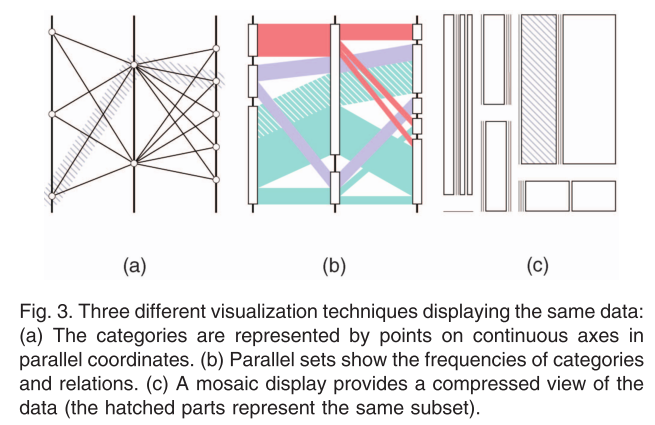
\includegraphics[width=0.8\textwidth]{"_img/Parallel_Coordinates_1.png"}
		\caption{Parallel Coordinates}
		\label{fig:parallelcoordinates1}
	\end{figure}

	Parallel Set是一种可视化技术,还是一种交互框架。
	它能够很自然的将类别变量映射到可视实体上,这使得交互分析更有效率。

	\subsection{交互(图\ref{fig:parallelcoordinates2})}
	\begin{framed}
		Shneiderman’s visual information seeking mantra:
		\textcolor{red}{overview first, zoom and filter, then details-on- demand}
	\end{framed}
	\begin{itemize}
		\item 选择高亮
		\item 交互查询
		\item 过滤
		\item 维度和分类重排
	\end{itemize}
	\begin{figure}[h]
		\centering
		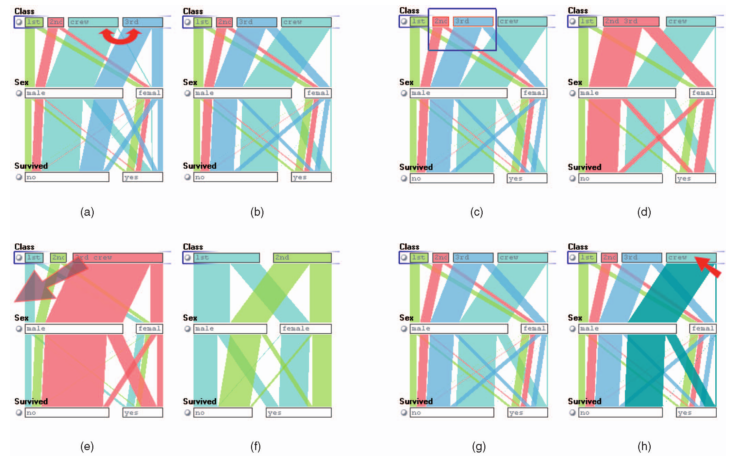
\includegraphics[width=\textwidth]{"_img/Parallel_Coordinates_2.png"}
		\caption{a分类重排,b重新布局layout,c合并分类,d层次分析,e去除分类,f过滤,g高亮,h多维关系}
		\label{fig:parallelcoordinates2}
	\end{figure}

	\fbox{用户选择感兴趣的数据}$\longrightarrow$
  \fbox{探索数据间的关系}$\longrightarrow$
  \fbox{选择数据创建新的View(Dimension)}		

	\subsection{其他}
	对于不是分类属性的维度,比如说连续属性,需要将其分段划分。

	坐标轴的顺序可能会影响数据的探索。

	对于层次数据,每一层可以作为一个坐标轴来进行分类,每层的不同类型的节点作为不同的分类。

	\section{Ordered and Quantum Treemaps: Making Effective Use of
		2D Space to Display Hierarchies\cite{Bederson2002}}
		文章提出了两种treemap算法,ordered-treemap和quantum-treemap。
		\begin{itemize}
			\item ordered-treemap算法用来解决一般treemap算法中节点位置突变的问题。
				在普通的算法中,当数据发生细小的变化时往往造成treemap结构的很大变化。
				ordered-treemap算法使得数据中相邻的节点在生成的treemap中依旧相邻(或不会相隔很远),
				所以当数据属性发生变化时,整个图结构不会发生很大的变化。
			\item quantum-treemap用来显示fixed-size objects,如图片。
				在显示图片时需要保证图片的aspect-ratio, squarified-treemap可以作为一个候选,
				但是它能够在一定程度上保证横纵比,但是无法保证fixed-size object的固横纵比。
		\end{itemize}

		\section{Multitrees: Enriching and Reusing Hierarchical Structure\cite{Furnas1994}}
		文章引入了multitree这种结构来展示信息。Multitrees是一类带有unusual properties的DAG,
		把树作为其子结构增加了它的可视别性。
		在层次上下文交换或者在一个层次重用的模型中,这些子树具有自然的语义解释
		(These subtrees have a natural semantic interpretation pro- viding alternate hierarchical contexts for information, as well as providing a natural model for hierarchical reuse)
		Multitrees中的子树提供基于树的图交互。

		DAG可以表示抽象的语义概念:比如父类子类(class above subclass)、聚合部分(aggregations above subparts)。
		DAG的问题在于其结构很难布局并理解,即使很简单的邻居关系就可能造成非平面的布局,导致边的交错。
		\subsection{Motivation}

		\begin{itemize}
			\item 寻找一种介于DAG和tree的结构,在展现信息上提供一种新的选择。
			\item reuse of hierarchical structure.对于公司具有的文档树,每个职员可能需要自定义符合自己需求的结构,
				职员大多不需要这么一个大的聚合文档结构,而是需要在小视图中寻找自己需要的部分。
				这就需要一种能够把树的片段重构成新的树结构的途径。\ref{fig:multitree_1}
		\end{itemize}
		\begin{figure}[h]
			\centering
			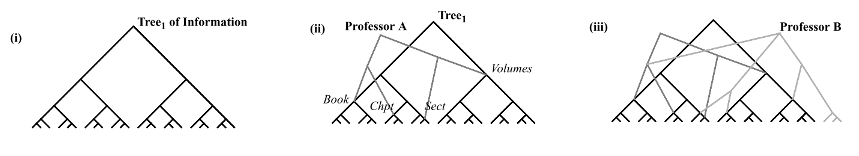
\includegraphics[width=\textwidth]{_img/Multitrees_1.png}
			\caption{Example for hierarchy reuse}
			\label{fig:multitree_1}
		\end{figure}

		\section{Voronoi Treemaps\cite{Balzer2005}}
		该论文提出的方法将treemap构成的基本元素从矩形拓展到了任形状,从而消除了一般treemap采用矩形时出现的横纵比不均衡以及不能清楚的展示数据的层次结构等问题。
		所以Voronoi Treemap更具灵活性,能够在更多的应用中使用。
		层次结构经常用作数据的分类、排序、组织的一种抽象,被广泛应用在多种数据中。
		(Hierarchical structures are an often used abstraction for the classification, 
		sorting, and organization of a broad variety of data.)
		Treemap具有的space-efficiency特性,使得它被广泛应用在系谱图(family tree)、文件系统的组织结构、软件架构、
		金融分析、体育报告等多种领域。

		文章中的Voronoi Treemap的基础是centroidal voronoid tessellation\cite{du1999centroidal}的使用。这个技术被广泛应用在能量最小化的各个领域,比如
		数据压缩,图像处理,网格细化(mesh refinement),资源分配以及科学可视化中。
		\begin{figure}
			\centering
			\begin{subfigure}[h]{0.5\textwidth}
				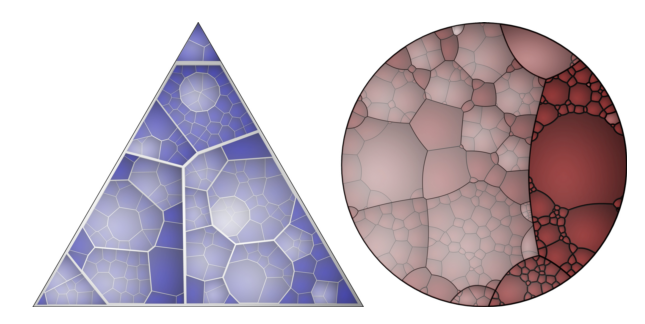
\includegraphics[width=0.8\textwidth]{_img/VoronoiTreemap_1.png}
				\label{fig:voronoi_treemap_1}
			\end{subfigure}

			\begin{subfigure}[h]{0.5\textwidth}
				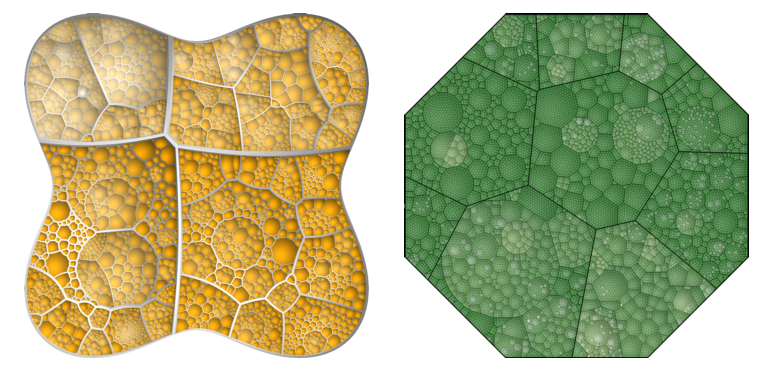
\includegraphics[width=0.8\textwidth]{_img/VoronoiTreemap_2.png}
				\label{fig:voronoi_treemap_2}
			\end{subfigure}
			\caption{Voronoi Treemap Examples}
		\end{figure}

		\section{Cheops: A Compact Explorer For Complex Hierarchies\cite{Beaudoin1996}}
		数据量的增多,加大了层次数据可视化的难度,一方面数据越来越复杂,另一方面数据的节点一层一层呈指数增长。
		一般的可视化技术能够有效的处理1000个几点左右的层次数据,一旦数据量超过5000,
		就需要一些特殊的技术来弥补数据量过大造成的节点重叠等问题,比如通过cluster来减少节点数目,再通过交互方式显示被隐藏的节点。
		但是cluster技术会影响可视结果的稳定性。

		文章提出了一个浏览大量复杂层次数据的可视技术,Cheops,可以处理1000万到10亿的节点数目。
		它能够在保持节点上下文环境的同时浏览节点的细节信息。

		传统的方法一般是在基本的表现形式上通过交互来加强信息的显示,最常用的是focus+context和fisheye。
		当这些方法用在比较复杂的数据上时会存在一些问题,
		比如因为使用了DOI(Degree-of-Intrest)函数使得周围的节点扭曲。当焦点改变的时候有可能需要重绘整个视图,
		效率就会有所下降。

		\subsection{论文大意}
		Cheops方法使用三角形作为可视的基本元素,通过元素重叠的方式节省空间,如图\ref{fig:Cheops_1}。
		然后通过交互手段根据需要选择性的显示重叠的节点。在实际中节点并不是完全重叠。

		\begin{figure}[h]
			\centering
			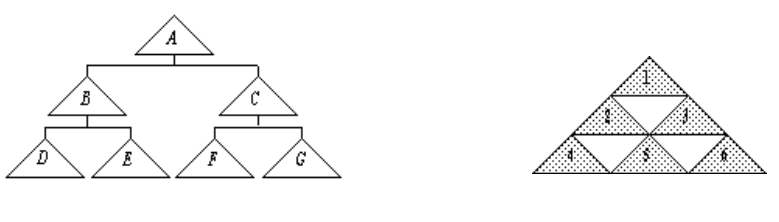
\includegraphics[width=0.8\textwidth]{_img/Cheops_1.png}
			\caption{从做图到右图的转换,左图中的EF两个节点在右图中重叠为节点5}
			\label{fig:Cheops_1}
		\end{figure}

		为了能够在动态的上下文中浏览节点,实现中使用了\emph{selecton}和\emph{pre-selection}技术。

		\begin{itemize}
			\item selection操作是说当用户选中一个节点(logical node)时,高亮显示以整个
				节点为根的树,其余的节点只显示一个轮廓如图\ref{fig:Cheops_2}左。旁边面板显示每个层次中选中的点的信息。
			\item pre-selection是说用户选中一个节点后,随机的选择一个用户可能选择的子节
				点,用户通过鼠标操作可以在子节点中进行切换,如图\ref{fig:Cheops_2}右。
		\end{itemize}

		\begin{figure}[h]
			\centering
			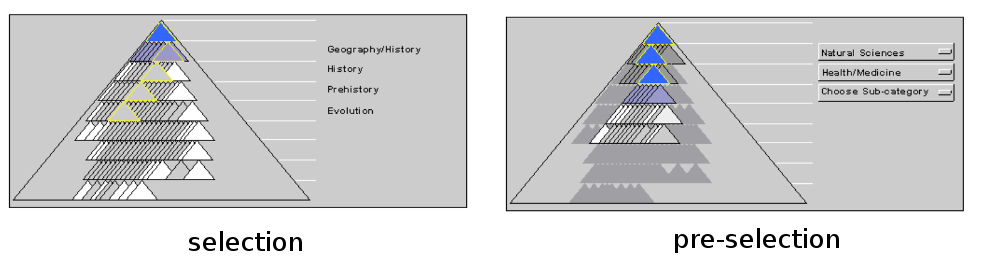
\includegraphics[width=0.8\textwidth]{_img/Cheops_2.png}
			\caption{selection和pre-selection}
			\label{fig:Cheops_2}
		\end{figure}

		这两种选择方式能够让用户在复杂的层次结构中快速的定位到节点。

		另为除了在图上选择点以外,旁边面板提供的类似comb select的方式来选择节点,
		图的下方也有navigation button来帮助用户选择。

		其他的交互slider、bookmarks、histogram。
		bookmarks允许用户保存某个视图,histogram用户显示节点或者当前选中结构的信息。
		如图\ref{fig:Cheops_3}

		\begin{figure}[h]
			\centering
			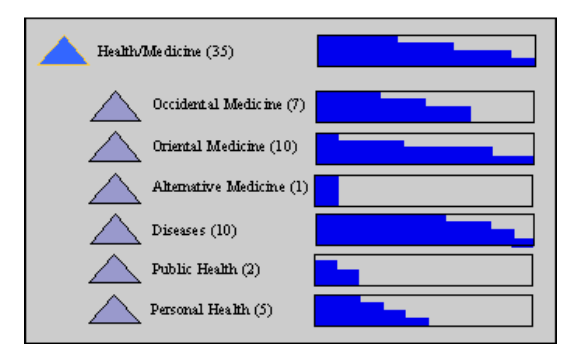
\includegraphics[width=0.8\textwidth]{_img/Cheops_3.png}
			\caption{图中可以看出,通过比较,disease节点应该是用户关注的下一个节点}
			\label{fig:Cheops_3}
		\end{figure}

		\subsection{缺点}

		这个方法适合在大量数据中查找信息或者查看数据的结构特性。
		在对数据属性的显示上呈现的效果不是很丰富,所以不适合用于数据的比较或者查看数据属性之间的关系。

		\subsection{启发}

		\begin{enumerate}
			\item 交互中,同一个功能可能需要多种方式实现来方便不同用户或者在不同的状态下进行选择。
			\item 交互不是目的,交互是为了方便用户提取图中的信息。
				所以可以以一种\emph{显示->交互->信息提取->显示->交互->信息提取}的循环模式逐步让用户提取信息。
		\end{enumerate}

		\subsection{思考}
		overlap的方式在什么情况下适用?缺点?优点?

		\bibliographystyle{plain}
		\bibliography{ref_readings}
		\end{document}
